\subsection{Experimental design}
\subsubsection{Participants}
Sixteen people, ten males and seven females, participated in the experiment (mean age = 24.35, SD = 6.87). 
\subsubsection{Materials}
For the experiment a computer was used to present the visual stimuli and feedback to the participant. A LEAP motion and a keyboard + mouse were used as input modalities for the participant. Furthermore, a lamp was used to hang the LEAP motion upside down.
\subsubsection{Task and procedure}
For this experiment participants were sitting behind a computer screen. In front of the screen there was a keyboard and a mouse, and on the right (or left for left-handed participants) there was a lamp with a leap motion attached to it (see Figure~\ref{fig:configuration}).

The experiment consisted of two sessions: a LEAP-motion session (in which participants used the LEAP motion interface) and a keyboard \& mouse session (in which participants used the keyboard \& mouse interface). The order of the sessions was counterbalanced.

Before the experiment participants received instructions about the task they were going to perform. Before every session participants received instructions about how to use the interface: which actions are possible, how to perform the actions (LEAP motion: possible gestures, keyboard + mouse: which keyboard and mouse button to use). After these instructions participants got 3 minutes to explore the interface that they were going to use in the upcoming session. 
Both sessions consisted of 3 trials. In each trial the participant had to replicate a target model. The target model was presented in the right corner of the screen as a 2-D matrix (see Figure~\ref{fig:environment} and Appendix C). In the LEAP motion session participants had to replicate the target models by by making gestures, while in the keyboard \& mouse session they had to do this by using the keyboard and the mouse. For every trial there was a time limit of 5 minutes. Participants were informed about this in the instructions.

After a session participants filled in a Post-Study System Usability Questionnaire about the interface they used in that session (see Appendix A). 
For possible follow-up analyses the participants were, after the two sessions, asked to fill in a questionnaire about their preferences, background and previous experience and/or expertise with the two interfaces (see Appendix B). Please find a overview of the experiment routine in Figure~\ref{fig:experimentroutine}.
\begin{figure}
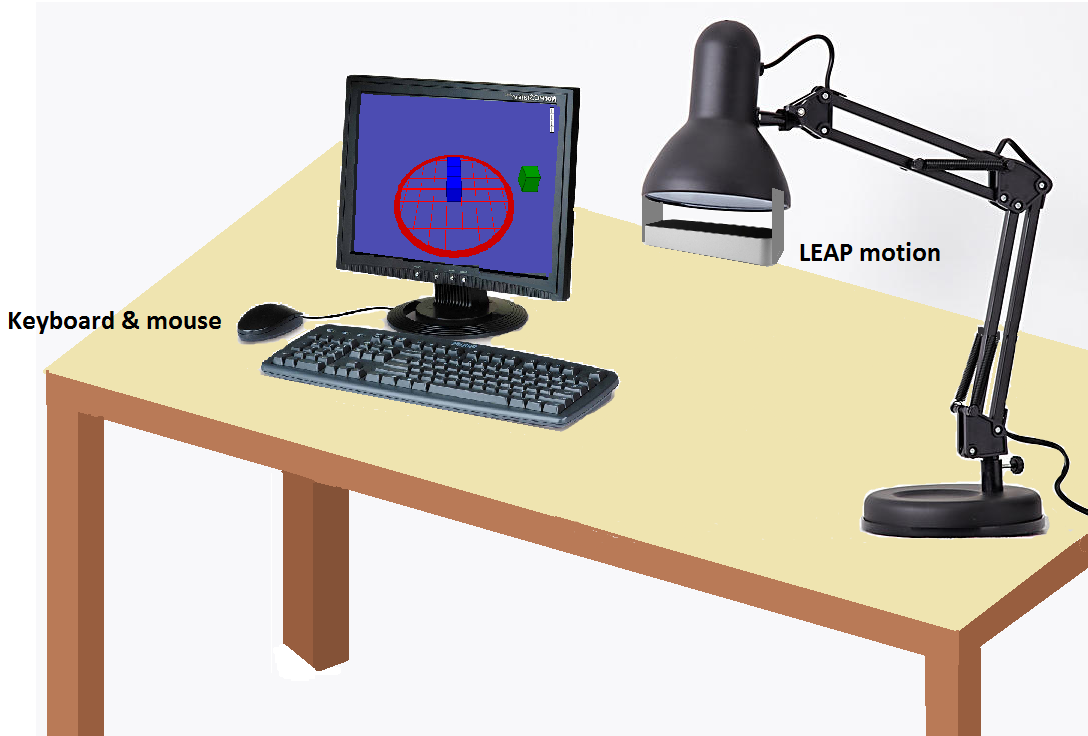
\includegraphics[width=\textwidth]{imgs/configuration}
\caption{Overview of the arrangement of the materials during the experiment.}
\label{fig:configuration}
\end{figure}

\begin{figure}
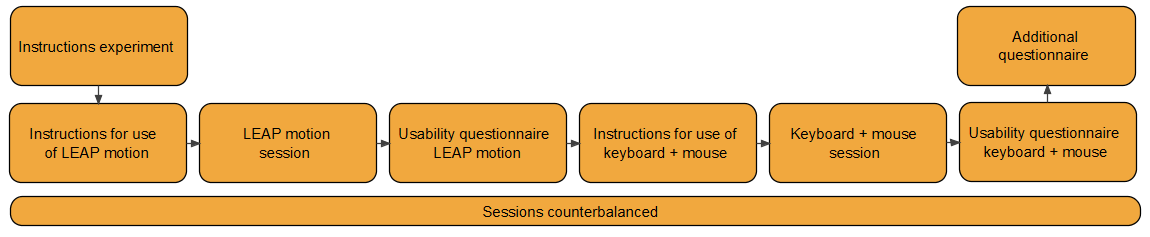
\includegraphics[width=\textwidth]{imgs/experimentroutine}
\caption{Overview of the experiment routine. The LEAP motion session and keyboard + mouse session were counterbalanced.}
\label{fig:experimentroutine}
\end{figure}


\subsubsection{Measurements}
In this experiment several measurements were done using a logger and questionnaires. 

Usability was measured using the Post-Study System Usability Questionnaire (PSSUQ) questionnaire ~\cite{lewis1992psychometric}. Items are displayed with seven-point graphic scales with on the end points the terms “Strongly agree” for 1 and “Strongly disagree” for 7, and a “Not applicable” (N/A) point next to the scale. The PSSUQ was adapted to better fit with our system. questions 9-15 (measuring Information Quality) were excluded considering that our interfaces did not differ with respect to information provided. Furthermore, help or error messaging was neither used or necessary in our system. The adapted PSSUQ is attached in Appendix A. This questionnaire now measures three system qualities: Overall quality, System Usefulness and Interface quality.  Different items on the questionnaire respond to different system qualities:
\begin{itemize}
	\item Overall satisfaction: Average the responses to Items 1 through 12.
	\item System usefulness: Average the responses to Items 1 through 8.
    \item Interface quality: Average the responses to Items 9 through 11.
\end{itemize}

The logger that was build for this experiment logged all the actions done by the user. Using this logger several features were combined into variables: 
\begin{itemize}
	\item Accuracy: number of useful moves/total number of moves.
	\item Average speed: average number of frames over three trials.    
	\item Distance travelled: distance travelled with the interaction device.
    \item Block repositioning: number of block replacements.
    \item Orientation changes: sum of horizontal and vertical rotations.
\end{itemize}


\subsubsection{Design}
The experiment was done and analysed using a within-subject design with as independent variable Interface (LEAP motion, keyboard \& mouse) and with as dependent variables: Overall satisfaction, System usefulness, Interface quality, Accuracy, Average speed, Distance travelled, Block repositioning, Orientation changes. 

